\begin{figure}
    \centering
    \begin{subfigure}{\linewidth}
    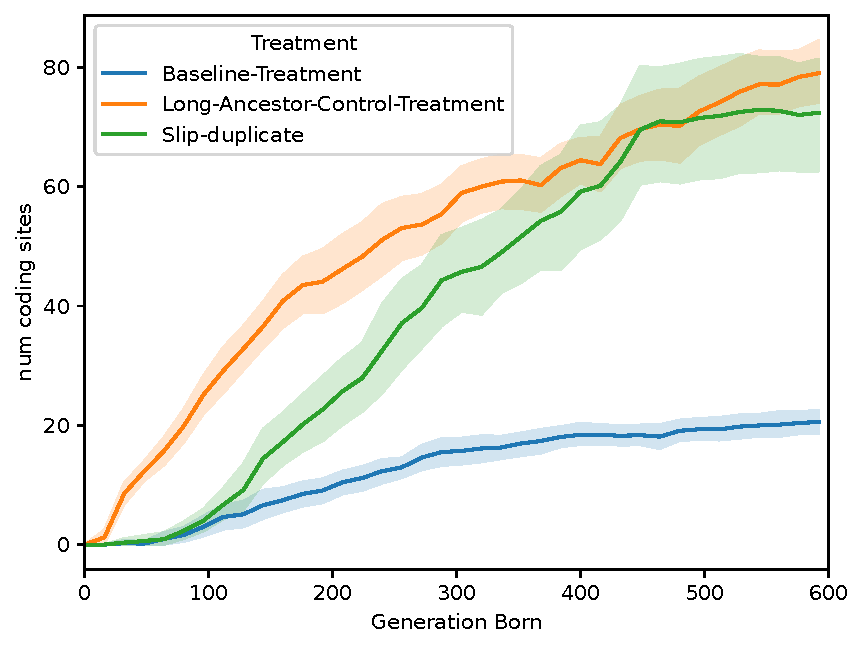
\includegraphics[width=\linewidth]{binder/binder/teeplots/hue=treatment+post=plt-xlim-0-600+viz=lineplot+x=generation-born+y=num-coding-sites+ext=.pdf}
    \caption{\footnotesize active coding sites}
    \label{fig:num-coding-sites:active}
    \end{subfigure}

    \begin{subfigure}{\linewidth}
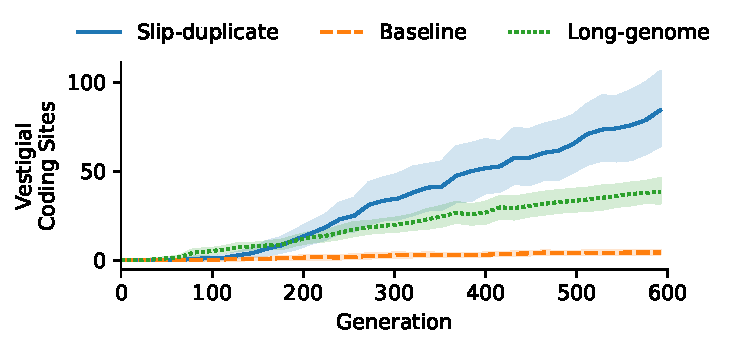
\includegraphics[width=\linewidth,clip, trim=0 0 0 0.8cm]{binder/binder/teeplots/hue=treatment+post=plt-xlim-0-600+viz=lineplot+x=generation-born+y=num-free-sites+ext=.pdf}
    \caption{\footnotesize vestigial coding sites}
    \label{fig:num-coding-sites:vestigial}
    \end{subfigure}
    \caption{
        \textbf{Gene duplication boosts accumulation of vestigial coding sites.}
        \footnotesize
        Generation-by-generation counts of coding sites over evolutionary history.
        Here, ``active'' coding sites refer to genome instructions determined through knockout to contribute to fitness with respect to self-copy viability or a rewarded phenotypic trait.
        As shown in panel \ref{fig:num-coding-sites:active}, gene duplication yields active coding site counts comparable to long-genome control.
        Vestigial coding site count, by contrast, reports the number of sites determined to have contributed to fitness in an ancestor, but are no longer active coding sites.
        As shown in panel \ref{fig:num-coding-sites:active}, vestigial coding site count under slip-duplication treatment outpace control treatments.
        Error bands give 95\% CI, bootstrapped over 30 replicates per treatment.
    }
    \label{fig:num-coding-sites}
\end{figure}
